\documentclass[10.5pt]{config}
% 本实验报告采用 署名-相同方式共享 4.0 国际许可协议 (CC BY-SA 4.0)
\usepackage{multirow}
\usepackage{wrapfig}
\usepackage{setspace}
\usepackage{titlesec}
\usepackage{ctex}
\usepackage{graphicx} % 用于插入图片
\usepackage{float}    % 用于控制图片位置
\usepackage{makecell}

\titleformat{\subsubsection}[block]  % 设置为块级标题（自动换行）
{\normalfont\bfseries}{\thesubsubsection}{1em}{} 
\titlespacing*{\subsubsection}{1.5em}{3.25ex}{1.5ex}  % 调整缩进：左缩进2em
\setstretch{1.5}

% --- 请在这里填写您的个人信息 ---
\major{机械工程} % 专业
\name{韩颂义}
\partner{} % 签名栏
\stuid{3240104198}
\date{3.12}
\lab{东3-208}
\grades{}
\course{电工电子学实验}
\instructor{季瑞松} % 指导老师
\exptype{基础实验} % 实验类型
\expname{电路元件伏安和电源外特性测量} % 实验名字


\begin{document}

\makeheader % 首页头部

\section{实验目的和要求}

\begin{enumerate}[label=\arabic*., leftmargin=2em]
    \item 掌握函数信号发生器和示波器的使用。
    \item 理解掌握电路元件伏安特性定义。
    \item 掌握线性电阻和非线性电阻元件伏安特性的测量。
    \item 掌握电源外特性的测量。
\end{enumerate}

\section{实验内容和原理}


\subsection{实验原理}

\subsubsection*{1.1 测量电路元件的伏安特性}

伏安特性是指元件两端所加的电压与通过它的电流之间的关系。用纵坐标表示电流 $i$、横坐标表示电压 $u$，以此画出的 $i-u$ 图像叫作元件的伏安特性曲线图。

电阻元件有线性电阻和非线性电阻。线性电阻两端的电压与通过它的电流成正比，其伏安特性曲线为过原点的直线，不管流过的电流大小，其电阻值是不变的；非线性电阻两端的电压和流过它的电流不呈线性关系，阻值是变化的。图1、2为电路元件伏安特性测量电路，其中 $U_S$ 为可调电压源大小，$R_A$、$R_V$ 分别为电流表和电压表的内阻值，$R_X$ 为被测元件电阻大小。图中，$R_S$ 限流电阻的作用是保证电源和被测元件正常工作，满足其额定功率要求。为减小测量误差，通常，当 $R_X \ll R_V$ 时采用图1所示电路；当 $R_X \gg R_A$ 时，采用图2所示电路。

\begin{figure}[H]
    \centering
    % 左侧图片
    \begin{minipage}[b]{0.3\textwidth}
        \centering
        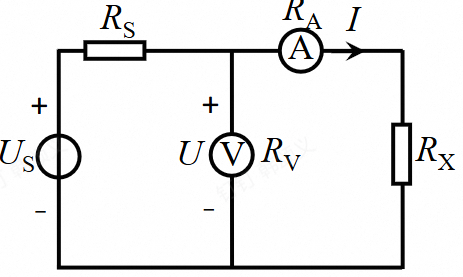
\includegraphics[width=\textwidth]{figures/neijie.png}
        \caption{电流表内接法}
        \label{fig:inner}
    \end{minipage}
    \hfill % 在两个小页之间填充弹性间距
    % 右侧图片
    \begin{minipage}[b]{0.3\textwidth}
        \centering
        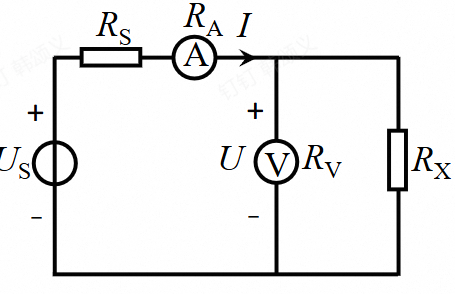
\includegraphics[width=\textwidth]{figures/waijie.png}
        \caption{电流表外接法}
        \label{fig:outer}
    \end{minipage}
\end{figure}

\subsubsection*{1.2 测量电源的外特性}

一个实际的电压源可以用一个大小为 $U_S$ 的理想电压源和一个阻值为 $R_S$ 的电阻串联来等效。电源的端电压 $U$ 和端电流 $I$ 的关系为
$$ U = U_S - R_S I $$
即为电压源的外特性曲线。测量电路如图3所示。

同样，实际的电流源可以用一个大小为 $I_S$ 的理想电流源和一个阻值为 $R_S$ 的电阻的并联来等效，电源的端电流 $I$ 与端电压 $U$ 的关系为
$$ I = I_S - \frac{1}{R_S} U $$
即为电流源的外特性曲线。测量电路如图4所示。


\begin{figure}[H]
    \centering
    % 左侧图片
    \begin{minipage}[b]{0.48\textwidth}
        \centering
        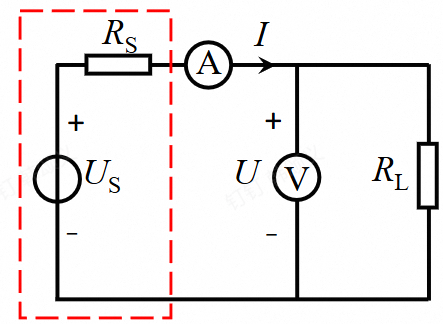
\includegraphics[width=\textwidth]{figures/dianya.png}
        \caption{电压源外特性}
        \label{fig:inner}
    \end{minipage}
    \hfill % 在两个小页之间填充弹性间距
    % 右侧图片
    \begin{minipage}[b]{0.48\textwidth}
        \centering
        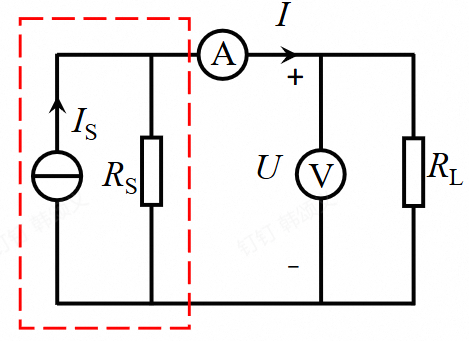
\includegraphics[width=\textwidth]{figures/dianliu.png}
        \caption{电流源外特性}
        \label{fig:outer}
    \end{minipage}
\end{figure}



\section{主要仪器设备}
\begin{enumerate}[label=\arabic*., leftmargin=2em]
    \item 电工电子综合实验台。
    \item 电阻元件、十进制电阻箱、二极管。
    \item 双踪数字示波器。
    \item 函数信号发生器。
\end{enumerate}

\section{操作方法和实验步骤}

\subsection*{1. 测量电路元件的伏安特性}
按图1接线，其中线性电阻 $R_X = 1k\Omega$，限流电阻 $R_S = 100\Omega$；缓慢调节可调电压源输出电压 $U_S$，分别测出线性电阻的电压值 $U$ 和电流值 $I$，测量结果记入表1。将线性电阻替换为整流二极管，将测量结果记入表2。

\subsection*{2. 电压源外特性测量}
按图3所示接线，其中 $U_S = 10\,\mathrm{V}$，$R_S = 100\Omega,\mathrm{\Omega}$，改变负载电阻值 $R_L$，将测量数据记入表3。

\subsection*{3. 电流源外特性测量}
按图4所示接线，其中 $I_S = 18\,\mathrm{mA}$，$R_S = 100\Omega,\mathrm{\Omega}$，改变负载电阻 $R_L$，将测量数据记入表4。


\section{实验数据记录和处理}
\subsection{数据记录}

\begin{table}[H]
    \centering
    \label{tab:linear_resistor_characteristic} % 改了标签名，防止 multiply defined
    % 使用 resizebox 确保表格不会超出边距
    \resizebox{\textwidth}{!}{
        % 修正为 10 列
        \begin{tabular}{|c|c|c|c|c|c|c|c|c|c|}
            \hline
            & $U/\mathrm{V}$（参考值） & 0 & 1 & 2 & 4 & 6 & 8 & 10 & 20  \\
            \cline{2-10}
            线性电阻 & $U/\mathrm{V}$ & 0 & 0.872 & 1.739 & 3.617 & 5.424 & 7.21 & 9.02 & 18.02  \\
            \cline{2-10}
            & $I/\mathrm{mA}$ & 0 & 0.872 & 1.745 & 3.60 & 5.42 & 7.24 & 9.02 & 18.16\\
            \hline
        \end{tabular}
       
    }
    \caption{线性电阻的伏安特性}
\end{table}

\begin{table}[H]
    \centering
    \label{tab:linear_resistor_characteristic} % 改了标签名，防止 multiply defined
    % 使用 resizebox 确保表格不会超出边距
    \resizebox{\textwidth}{!}{
        % 修正为 10 列
        \begin{tabular}{|c|c|c|c|c|c|c|c|c|c|c|c|c|}
            \hline
            & $U/\mathrm{V}$（参考值） & 0 & 0.2 & 0.4 & 0.6 & 1 & 2 & 5 & 10 & 20 & 50 & 80   \\
            \cline{2-13}
            整流二极管 & $I/\mathrm{mA}$ &  & 0.304 & 0.446 & 0.655 & 1.067 & 2.00 & 5.05 & 10.11 & 19.7 & 49.9 & 79.8  \\
            \cline{2-13}
            & $U/\mathrm{V}$ & 0.416 & 0.449 & 0.461 & 0.475 &0.492 & 0.518 & 0.561 & 0.599 & 0.639 & 0.700 & 0.732 \\
            \hline
        \end{tabular}
        
    }
    \caption{整流二极管的伏安特性}
\end{table}


\begin{table}[H]
    \centering
    \begin{tabular}{|c|c|c|c|c|c|}
        \hline
        $R_L/\Omega$ & 200 & 100 & 50 & 20 & 0 (短路) \\
        \hline
        $R_L/\Omega（实测值）$ & 200.6 & 101.5 & 51.5 & 21.7 & 1.0 \\
        \hline
        $U/\mathrm{V}$ & 6.61 & 4.95 & 3.30 & 1.66 & / \\
        \hline
        $I/\mathrm{mA}$ & 32.7 & 49.2 & 65.3 & 81.8 & 98.0 \\
        \hline
    \end{tabular}
    \caption{电压源的外特性}
    \label{tab:voltage_source_characteristic}
\end{table}

\begin{table}[H]
    \centering
    \begin{tabular}{|c|c|c|c|c|c|}
        \hline
        $R_L/\Omega$ & $\infty$（断路） & 100 & 50 & 20 & 0 (短路) \\
        \hline
        $R_L/\Omega（实测值）$ & / & 101.5 & 51.5 & 21.7 & 1.0 \\
        \hline
        $U/\mathrm{V}$ & 1.84 & 0.892 & 0.587 & 0.292 & / \\
        \hline
        $I/\mathrm{mA}$ & / & 8.85 & 11.65 & 14.44 & 17.51 \\
        \hline
    \end{tabular}
    \caption{电流源的外特性}
    \label{tab:voltage_source_characteristic}
\end{table}

\subsection{数据处理}

\begin{figure}[H] % [H] 表示强制图片停留在代码所在位置
    \centering
    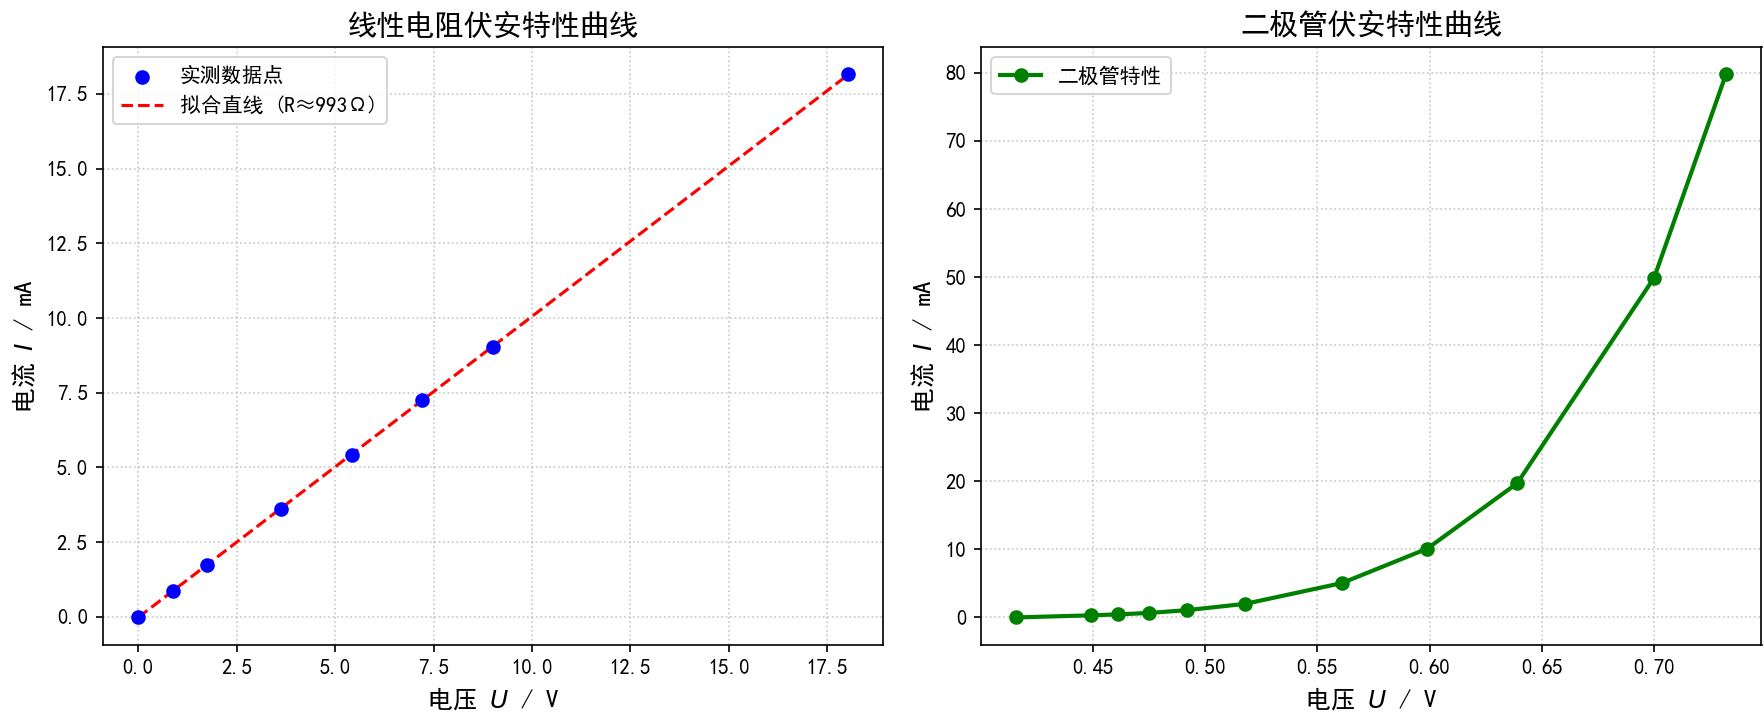
\includegraphics[width=0.8\textwidth]{figures/texin.png} % 替换为你的文件名，width可调节大小
    \caption{线性电阻和二极管的伏安特性曲线}
    \label{fig:experiment_circuit} % 图片引用标签，需唯一
\end{figure}

\begin{figure}[H] % [H] 表示强制图片停留在代码所在位置
    \centering
    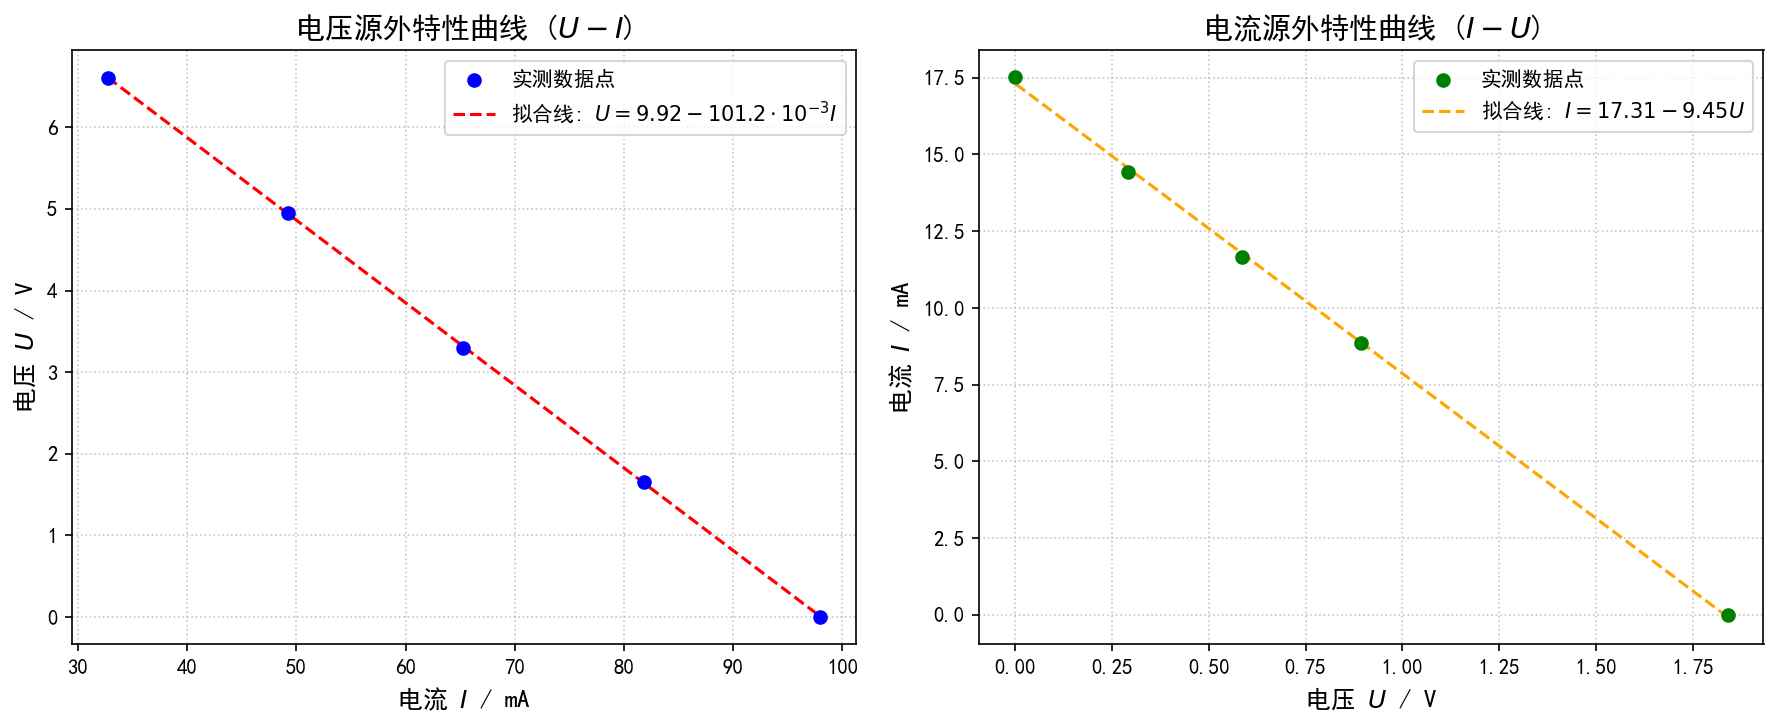
\includegraphics[width=0.8\textwidth]{figures/waite.png} % 替换为你的文件名，width可调节大小
    \caption{电流源和电压源的外特性曲线}
    \label{fig:experiment_circuit} % 图片引用标签，需唯一
\end{figure}
\section*{六、实验结果与分析}

\subsection*{1. 电路元件的伏安特性分析}
\textbf{（1）线性电阻：}
根据表1的测量数据及图5的“线性电阻伏安特性曲线”可知，该电阻元件的电流 $I$ 与两端电压 $U$ 呈明显的正比例关系，其伏安特性曲线为过原点的直线。通过对实测数据点进行最小二乘法线性拟合，得到该电阻的阻值约为 $993\ \Omega$。该拟合值与实验设定的标称值 $1\ \text{k}\Omega$ 非常接近，充分验证了欧姆定律。测量存在的微小误差主要来源于测量仪表（电压表和电流表）自身的内阻分流/分压影响以及人为读数误差。

\textbf{（2）整流二极管：}
根据表2及图5的“二极管伏安特性曲线”可以看出，整流二极管呈现典型的非线性特征。当正向电压较低时，通过二极管的电流极小，几乎为零；当正向电压超过阈值电压（实验测得约0.416$\Omega$）后，随着电压的微小增加，电流呈指数级急剧上升。这充分验证了二极管的单向导电性及其非线性伏安特性的客观规律。

\textbf{（3）电流表外接法误差分析：}
在本实验测量线性电阻与二极管时，均采用了电流表外接法（如图2所示）。由线性电阻测量结果为$993\Omega$，比标称阻值小，这符合电流表外接法的特点，即测出来的实际电阻是线性电阻和电压表电阻的并联电阻。
\subsection*{2. 电源的外特性分析}
\textbf{（1）电压源外特性：}
根据表3和图6中的“电压源外特性曲线（$U-I$）”，实际电压源的端电压 $U$ 随着输出电流 $I$ 的增大而呈线性下降趋势。对实验数据进行拟合得到方程：$U = 9.92 - 101.2 \times 10^{-3} I$。将此拟合结果与电压源外特性理论方程 $U = U_S - R_S I$ 对比，可计算出实际测得的电压源电动势 $U_S \approx 9.92\ \text{V}$，等效内阻 $R_S \approx 101.2\ \Omega$。该测算结果与实验中实际接入的 $U_S = 10\ \text{V}$、$R_S = 100\ \Omega$ 高度吻合。

\textbf{（2）电流源外特性：}
根据表4和图6中的“电流源外特性曲线（$I-U$）”，实际电流源的输出端电流 $I$ 随着端电压 $U$ 的升高而线性减小。对数据点进行拟合得到方程：$I = 17.31 - 9.45 U$。将其与理论方程 $I = I_S - \frac{1}{R_S} U$ 对比，可得实际测量的电流源输出恒流 $I_S \approx 17.31 \text{mA}$，等效内阻 $R_S = \frac{1}{9.45} \text{ k}\Omega \approx 105.8\ \Omega$。该结果与理论设定的 $I_S = 18\text{ mA}$、$R_S = 100\ \Omega$ 存在轻微偏差，可能来源于测量仪表（如电压表和电流表）自身的内阻分压/分流影响，以及人为的读数误差 。但是从整体来看，结果依然在合理的准确范围内。
\section*{七、讨论、心得}

本次实验我们从电路元件的伏安特性，到电流源和电压源的外特性，从内到外剖析电路的电流电压关系。除了线性元件的分析，我们还进行了电流电压的动态分析，学习了示波器和信号发生器的使用方法，为以后更复杂的电路搭建和分析打好了基础。

\end{document}



